\documentclass[tikz,border=2pt]{standalone}
\usepackage{pgfplots}
\pgfplotsset{compat=1.7}

\begin{document}
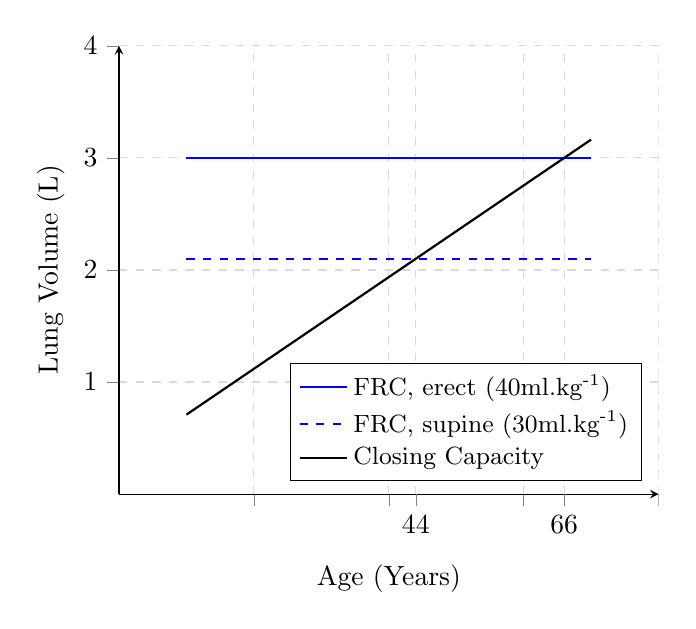
\begin{tikzpicture}

\tikzset{
    myarrow/.style={
        sloped,
        isosceles triangle,
        anchor=apex,
        fill=black,
        inner sep=2pt
    }
}
    \begin{axis}[
        axis lines=middle,
	ymin = 0,
	ymax = 4,
	xmin = 0,
xmax = 80,
        grid = major,
        grid style={dashed, gray!30},
	 ylabel near ticks,
	xlabel near ticks,
	  xticklabels={},
	extra x ticks={44, 66},
extra x tick labels = {44,66},
        xlabel=Age (Years),
        ylabel=Lung Volume (L),
        tick align=outside,
        enlargelimits=false,
legend pos=south east,
legend style={font=\small, cells={align=left}},
legend cell align={left}]

\addlegendimage{blue, thick}
\addlegendentry{FRC, erect (40ml.kg\textsuperscript{-1})}
\addlegendimage{blue, dashed, thick}
\addlegendentry{FRC, supine (30ml.kg\textsuperscript{-1})}

	\draw [blue, thick] (axis cs: 10, 3) -- (axis cs: 70,3) node[above] {};
	\draw [blue, thick, dashed] (axis cs: 10, 2.1) -- (axis cs: 70,2.1);
	\addplot[domain= 10:70, black, thick] {0.040909*x + 0.3};
\addlegendentry{Closing Capacity}

\end{axis}

\end{tikzpicture} 
\end{document}